\chapter{Các thuật toán trên đồ thị}
\section{Biểu diễn đồ thị trên máy tính}
\subsection{Ma trận kề}
Cho G = (V, E) là \textbf{đơn đồ thị} có n đỉnh 1, 2, \dots n và m cạnh. Ta có thể biểu diễn bằng một ma trận vuông cấp n với quy ước $A_{ij}=1$ hoặc true nếu có cạnh nối (i,j) và ngược lại $A_{ij}=0$ hoặc false. Nếu là đa đồ thị thì thay 1 thành số cạnh nối nó. Giá trị của $A_{ii}$ thì nên đặt theo mục đích nhưng nó thường được đật bằng 0.

Ưu điểm:
\begin{itemize}
    \item Dễ cài đặt, đơn giản, trực quan
    \item Để kiểm tra chỉ cần 1 phép so sánh
\end{itemize}
Nhược điểm:
\begin{itemize}
    \item Tốn bộ nhớ $O(n^2)$
    \item Không thể kiểm tra nhanh các đỉnh kề dẫn tới phí thời gian duyệt.
\end{itemize}
\subsection{Danh sách cạnh}
Ưu điểm:
\begin{itemize}
    \item Trong trường hợp đồ thị thưa (chẳng hạn m < 6n), nó sẽ tiết kiệm bộ nhớ vì chỉ cần 2m ô nhớ để lưu danh sách cạnh.
    \item Trong một số trường hợp khi ta phải xét tất cả các cạnh thì cài đặt danh sách cạnh sẽ làm cho việc duyệt dễ dàng hơn (thuật toán Kruskal chẳng hạn).
\end{itemize}
Nhược điểm: không thể duyệt nhanh tất cả các đỉnh kề với 1 đỉnh bất kì, ta buộc phải duyệt toàn bộ danh sách cạnh.
\subsection{Danh sách kề}
Để khắc phục yếu điểm của 2 cách biểu diễn trên, người ta đề xuất biểu diễn bằng danh sách kề. Trong danh sách này, với mỗi đỉnh v của đồ thị ta cho tương ứng với nó một danh sách gồm các đỉnh kề với nó.

Ưu điểm là dễ duyệt các đỉnh kề và các cạnh nhưng nhược điểm là khó có thể kiểm tra (u,v) là cạnh vì lúc đó ta phải duyệt toàn bộ các đỉnh kề với u.

\section{Duyệt đồ thị}
\subsection{Duyệt theo chiều sâu (Depth First Search - DFS)}
Tư tưởng của thuật toán đơn giản là, bắt đầu từ đỉnh u, ta tiếp tục duyệt các đỉnh kề với u, rồi lại tiếp tục duyệt như vậy đến khi không còn đường để đi bằng giải thuật đệ quy. Để không rơi vào vòng lặp vô tận (duyệt 1 đỉnh nhiều lần) ta đánh dấu đỉnh đó khi đi qua.

\begin{algorithmic}
    \Function{DFS}{u}
        \State $f_u\gets$ false
        \Comment{$f_v=$ true nếu đỉnh chưa thăm}
        \For{$v\in V$}
            \If{$f_v=$ true và $(u,v)\in E$}
                \State\Call{DFS}{v}
            \EndIf
        \EndFor
    \EndFunction
\end{algorithmic}

DFS trả về đường đi có thứ tự từ điển nhỏ nhất.

\subsection{Duyệt theo chiều rộng (Breadth First Search - BFS)}
Phương pháp này ưu tiên duyệt các đỉnh kề với nó hơn là tiếp tục duyệt theo chiều sâu như DFS. Với mọi đỉnh nó sẽ đẩy các đỉnh kề với nó vào danh sách chờ duyệt và duyệt theo thứ tự đến khi hết hàng chờ. Kết quả của việc này chính là duyệt theo chiều rộng.

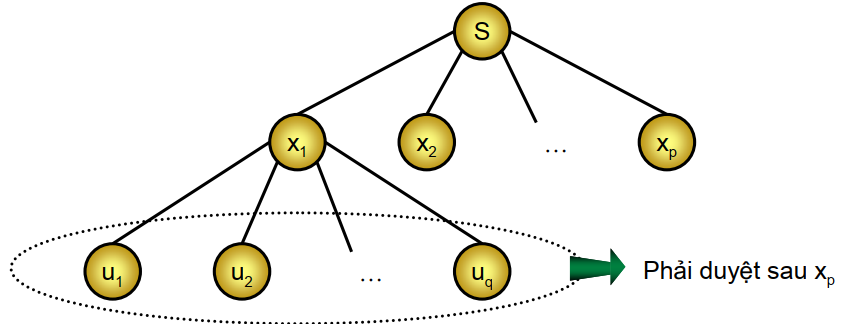
\includegraphics[scale=0.45]{dothi/bfs.png}

\begin{algorithmic}
    \Function{BFS}{}
        \State $f_s\gets$ false
        \Comment{Khởi tạo mảng đánh dấu s đã được thăm}
        \State $q\gets{s}$
        \Comment{Khởi tạo hàng đợi q chỉ chứa s}
        \While{$q\neq\emptyset$}
            \State $u\gets$\Call{Pop}{}
            \Comment{Lấy từ hàng đợi ra đỉnh u}
            \For{$v\in V$}
                \If{$f_v=$ true và $(u,v)\in E$}
                    \State $f_v=$ false
                    \State\Call{Push}{v}
                    \Comment{Đẩy v vào hàng đợi}
                \EndIf
            \EndFor
        \EndWhile
    \EndFunction
\end{algorithmic}

BFS trả về đường đi đi qua ít cạnh nhất.

\subsection{Độ phức tạp của DFS và BFS}
\begin{itemize}
    \item Trong trường hợp cài đặt bằng danh sách kề, cả hai đều có độ phức tạp $O(V+E)$, là cách cài đặt tốt nhất.
    \item Nếu biểu diễn bằng ma trận kề thì độ phức tạp là $O(n^2)$.
    \item Nếu biểu diễn bằng danh sách cạnh, việc duyệt những đỉnh kề với u sẽ phải duyệt toàn bộ danh sách cạnh, đây là cách cài đặt tồi nhất, có độ phức tạp $O(nm)$.
\end{itemize}

DFS và BFS dùng để xây dựng cây khung của đồ thị, tìm các chu trình cơ sở của đồ thị, định chiều đồ thị, liệt kê khớp-cầu của đồ thị\dots

\section{Tính liên thông. Bao đóng và thuật toán Warshall}
Với đồ thị G = (V, E) người ta xây dựng đồ thị G' = (V, E') với yêu cầu: nếu trong G u có thể đến v thì G' có cạnh nối (u,v). Lúc này G' gọi là bao đóng của đồ thị G. Dễ thấy rằng:
\begin{itemize}
    \item Một đơn đồ thị vô hướng là liên thông khi và chỉ khi bao đóng của nó là đồ thị đầy đủ.
    \item Một đơn đồ thị vô hướng có k thành phần liên thông khi và chỉ khi bao đóng của nó có k thành phần liên thông đồ thị đầy đủ.
\end{itemize}

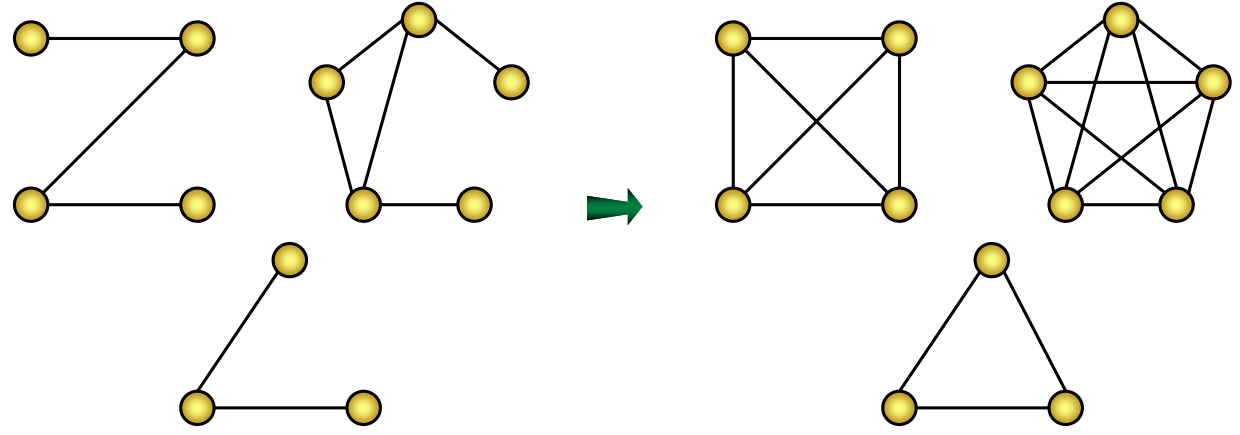
\includegraphics[scale=0.32]{dothi/baodong.png}

Thuật toán Warshall được xây dựng dựa trên định nghĩa: ta xét các cặp đỉnh (u, v): nếu có cạnh nối (u, k) và cạnh nối (k, v) thì ta nối thêm cạnh (u, v) nếu nó chưa có. Dễ thấy rằng có 3 biến chạy, độ phức tạp thời gian là $O(n^3)$.

\section{Thành phần liên thông mạnh}
Một đồ thị \textbf{có hướng} gọi là liên thông mạnh nếu như các đỉnh có thể đến được với nhau, ngược lại gọi là liên thông yếu nếu đồ thị vô hướng nền (bỏ đi các mũi tên) của nó là liên thông.

Diễn giải theo cách toán học hơn, đồ thị liên thông mạnh khi với mọi cặp đỉnh (u, v) ta có u đến được v và v đến được u, nhưng đồ thị liên thông yếu ta có u đến được v hoặc v đến được u.

\begin{figure}[h]
    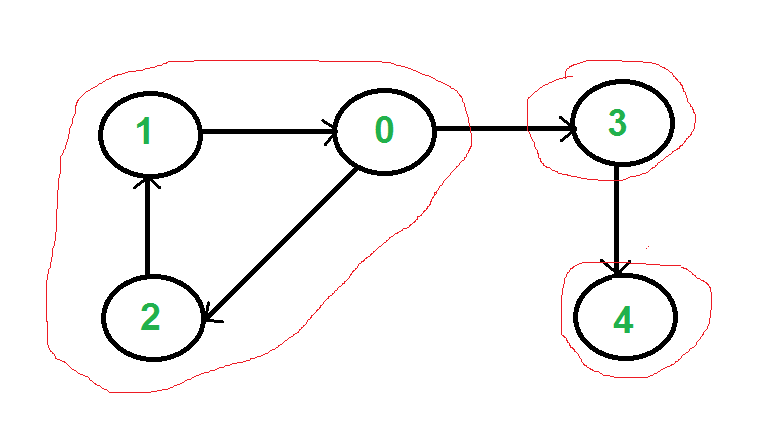
\includegraphics[scale=0.5]{dothi/ltmanh.png}
    \caption{Các thành phần liên thông mạnh}
\end{figure}

\subsection{Thuật toán Kosaraju}
Thuật toán Kosaraju xây dựng trên định nghĩa của TPLT mạnh, nó hoạt động như sau:
\begin{itemize}
    \item Sử dụng một ngăn xếp (stack) S, chọn V không thuộc S và gọi DFS(v). Đến đỉnh nào thì đẩy đỉnh đó vào S.
    \item Đảo ngược tất cả các cung.
    \item Lấy ra đỉnh trên cùng v của S. Tiếp tục gọi DFS(v). Các đỉnh có thể thăm lại được chính là các đỉnh thuộc TPLT mạnh chứa v. Ghi nhận và xoá chúng khỏi đồ thị cùng ngăn xếp S.
\end{itemize}
Cực kì đơn giản đúng không, dù độ phức tạp vẫn là O(V+E), tuy nhiên nó tốn 2 lần DFS, sẽ không hiệu quả bằng thuật toán Tarjan sắp được trình bày (chỉ tốn 1 lần DFS duy nhất), nó dựa trên rất nhiều cơ sở lí thuyết để sử dụng được.

\subsection{Một số khái niệm}
Trong cây DFS, nếu v đã được thăm trước u, có 3 khả năng xảy ra:
\begin{itemize}
    \item v là tổ tiên của u, DFS(u) do DFS(v) gọi tới. Cung (u, v) khi này gọi là \textbf{cung ngược}.
    \item v là con cháu của u, hay u đã được thăm trước v, nhưng DFS(u) sau khi đi theo hướng khác đã gọi DFS(v) rồi, nên khi đệ quy lùi lại DFS(u) sẽ thấy v là đã thăm. Lúc này cung (u, v) gọi là \textbf{cung xuôi}.
    \item v thuộc 1 nhánh cây DFS đã duyệt trước đó, hay sẽ có một đỉnh w được thăm trước cả u và v, nó rẽ sang nhánh khác thăm v trước xong rẽ sang nhánh này thăm u. Lúc này cung (u, v) gọi là \textbf{cung chéo}.
\end{itemize}
Hình bên dưới mô tả 3 cung này theo thứ tự từ trái qua phải.

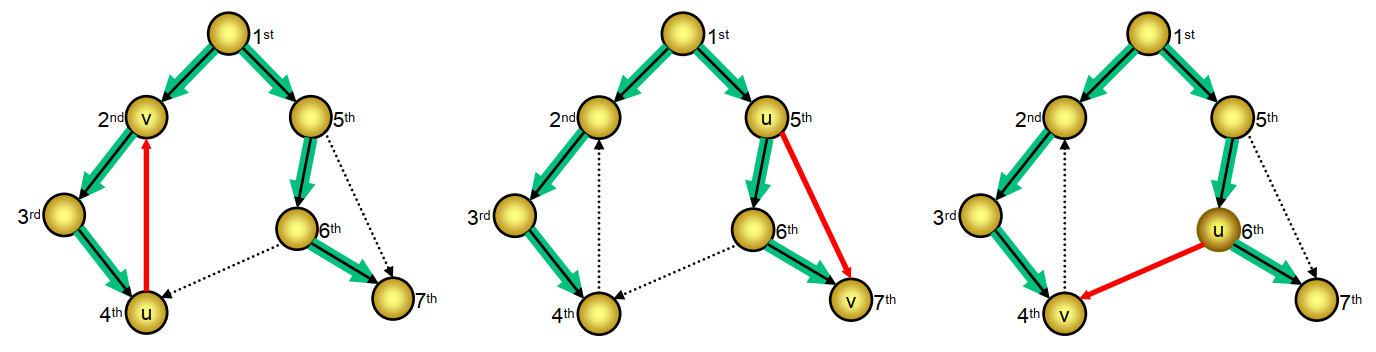
\includegraphics[scale=0.29]{dothi/cungxuoi_cungnguoc_cungcheo.png}

\subsection{Một số định lý và cơ sở lý thuyết}

\begin{theorem}
    Nếu a, b là 2 đỉnh thuộc TPLT mạnh C thì mọi đỉnh trên đường đi từ a tới b hoặc b tới a đều phải thuộc C.
\end{theorem}

Gọi v là đỉnh nằm trên đường đi từ a tới b. Nếu a muốn tới b, a phải đi qua v rồi đến b, và b muốn tới a theo con đường khác thì cũng phải đi qua v rồi mới tới a. Vậy v phải nằm trong TPLT mạnh đó.

\begin{theorem}
    Với một TPLT mạnh C bất kỳ, có một đỉnh r thuộc C sao cho mọi đỉnh của C đều thuộc nhánh DFS gốc r.
\end{theorem}

Gọi v là một đỉnh bất kỳ trong C khác r. Khi gọi DFS(r), tất cả các đỉnh kia sẽ phải thăm sau đỉnh r, rồi mới đến v. Vì v bất kỳ nên các đỉnh này phải thuộc nhánh DFS gốc r.

r còn được gọi là \textbf{chốt} của TPLT mạnh C. Trong cây DFS, chốt là đỉnh được thăm trước tất cả các đỉnh khác trong TPLT mạnh đó.

\begin{theorem}
    Nhánh DFS gốc a chỉ chứa một chốt duy nhất là a.
\end{theorem}

Với v nằm trong nhánh DFS gốc a, xét b là chốt của TPLT mạnh này. Ta sẽ chứng minh a trùng b. Nếu vậy, v cũng phải nằm trong nhánh DFS gốc b. Nếu a khác b thì có 2 khả năng:
\begin{itemize}
    \item Nhánh DFS gốc a chứa nhánh DFS gốc b, lúc này a sẽ thăm b, mâu thuẫn với giả thiết a sẽ không thăm được một chốt nào ngoài a.
    \item Nhánh DFS gốc a nằm trong nhánh DFS gốc b, hay a nằm trên đường đi từ b tới v. Theo định lý 1, a cũng phải thuộc TPLT mạnh đó, vậy nó có cả 2 chốt a và b, mâu thuẫn với khái niệm \textbf{chốt}.
\end{itemize}

Từ định lý 2 và 3 ta suy ra được: nhánh DFS gốc a chính là TPLT mạnh chứa a.

\subsection{Thuật toán Tarjan}
Chọn u là chốt mà DFS không thể tìm được chốt nào khác, ta thu được TPLT mạnh đầu tiên là nhánh DFS gốc u. Xoá nhánh này ra khỏi đồ thị, lại tìm thấy đỉnh v mà DFS không thể tìm được chốt nào khác, lại chọn TPLT mạnh thứ 2 là nhánh DFS gốc v. Tương tự với các TPLT mạnh còn lại. Có thể hình dung thuật toán này "bẻ" cây DFS tại các chốt thành các nhánh rời rạc, mỗi nhánh là một TPLT mạnh.

Nhưng cuối cùng vẫn còn một câu hỏi: Làm sao để biết v có phải chốt không? Để ý nhánh DFS gốc r.
\begin{itemize}
    \item Nếu từ các đỉnh thuộc nhánh DFS gốc r, không có cung ngược / chéo nào đi ra khỏi nhánh đó thì r là chốt. Nói cách khác, từ r chỉ có thể đến được các đỉnh thuộc nhánh DFS gốc r.
    \item Nếu từ đỉnh v của nhánh DFS gốc r có cung ngược lên đỉnh w là tổ tiên của r thì r không phải chốt.
    \item Nếu từ đỉnh v của nhánh DFS gốc r có cung chéo, ta sẽ thiết lập giải thuật sao cho khi đệ quy vừa lùi lại r, ta xoá ngay r khỏi đồ thị, vì nếu nó có chứa một chốt r' ở nhánh kia thì nó phải được duyệt rồi và bị xoá rồi, vì cung chéo sẽ chỉ đi tới nhánh thăm trước đó, chứ không đi sang nhánh thăm sau. Kể cả nếu r' là tiền bối của r thì r' phải đến được r, r có thể đến được nhánh DFS gốc r, vậy r' phải là chốt nên r không thể là chốt.
\end{itemize}

Từ 3 nhận xét trên ta rút ra được: r là chốt khi và chỉ khi không có cung nối từ một đỉnh thuộc nhánh DFS gốc r đến một đỉnh thăm trước r.

Thuật toán Tarjan xây dựng trên nhận xét này, nó đánh số cho cho các đỉnh theo thứ tự được thăm đầu tiên đến đỉnh thăm cuối cùng, gọi là \texttt{number[u]}. Ta tính thêm \texttt{low[u]} là giá trị number[\dots] nhỏ nhất trong các đỉnh đến được từ đỉnh v thuộc nhánh DFS gốc u bằng một cung (giả thiết rằng u có một cung giả nối với chính nó).

Cách tính \texttt{low[u]} như sau: Trước hết ta cho \texttt{low[u] = number[u]} hay u có cung tới chính u. Sau đó với mỗi đỉnh v nối từ u, có 2 khả năng:
\begin{itemize}
    \item Nếu v đã thăm: ta có \texttt{low[u] = min(low[u], number[v])}.
    \item Nếu v chưa thăm: ta gọi đệ quy thăm v sau đó tính \texttt{low[u] = min(low[u], low[v])}.
\end{itemize}

Dễ thấy rằng nếu \texttt{low[u] = number[u]} thì u là chốt vì không có đỉnh nào thăm trước nó.

\subsubsection{Đánh giá độ phức tạp}
Vì thuật toán Tarjan chỉ là sửa đổi một chút của thuật toán DFS bằng các thao tác O(1), nên độ phức tạp thời gian của nó bằng độ phức tạp thời gian của DFS.

\section{Bài toán đường đi ngắn nhất}
Đồ thị mà mỗi cạnh của nó được gán cho một số gọi là đồ thị có trọng số. Số gán cho mỗi cạnh gọi là trọng số của cạnh đó. Tương tự như đồ thị không trọng số thì cũng có nhiều cách biểu diễn đồ thị có trọng số trong máy tính, vd. với ma trận kề, nếu $c_{uv} = 1$ ta thay 1 thành trọng số của cạnh đó, còn nếu $c_{uv} = 0$, ta thay thành $+\infty$ hay $-\infty$, để nguyên 0\dots tuỳ thuộc vào thuật toán, sao cho dễ xử lý nhất. Quy ước $c_{vv} = 0$ với mọi v. Độ dài đường đi là tổng trọng số của các cạnh đã đi qua.

Ta sẽ chỉ xét đến đồ thị không có chu trình âm, vì nếu nó có chu trình âm (chu trình với độ dài âm), ta có thể đi qua nó vô hạn lần và mọi đường đi qua chu trình này đều sẽ có chi phí nhỏ nhất, để tránh trường hợp này người ta giải quyết bài toán \textbf{đường đi cơ bản ngắn nhất} (đường đi không có đỉnh lặp lại ngắn nhất), nhưng nó rất phức tạp.

\subsection{Thuật toán Ford - Bellman}
Có thể phát biểu cực kì đơn giản: Gọi $d_v$ là khoảng cách từ đỉnh bắt đầu s với $d_s=0$ và $d_v=+\infty\forall v\neq s$. Sau đó tối ưu hoá dần $d_v$ như sau, xét mọi cặp đỉnh u, v; nếu có bất kì cặp nào có $d_v>d_u+c_{uv}$ thì ta đặt lại $d_v=d_u+c_{uv}$. Nhớ rằng ta đặt $c_{uv}=+\infty$ nếu (u, v) không phải cung. Thuật toán kết thúc khi không thể tối ưu thêm bất kì $d_v$ nào được nữa.

\subsubsection{Tính đúng của thuật toán}
\begin{itemize}
    \item Tại bước khởi tạo thì $d_v$ là độ dài ngắn nhất từ s đến v không quá 0 cạnh.
    \item Giả sử khi bắt đầu bước i, $d_v$ bằng độ dài đường đi ngắn nhất từ s tới v không quá i - 1 cạnh, qua bước lặp nó sẽ kết nạp thêm đỉnh u vào đường đi này, vậy đường đi lúc này đã có i cạnh, suy ra được công thức trên.
    \item Sau bước lặp thứ n - 1, ta có $d_v$ là độ dài đường đi ngắn nhất không quá n - 1 cạnh, vì đồ thị không có chu trình âm nên sẽ có đường đi ngắn nhất là đường đi cơ bản (qua không quá n - 1 cạnh), vậy có không quá n - 1 bước.
\end{itemize}

Trong khi cài đặt chương trình nếu thuật toán có dạng:
\begin{minted}{cpp}
    for (int u = 1; u <= n; u++)
        for (int v = 1; v <= n; v++)
            d[v] = min(d[v], d[u] + c[u][v])
\end{minted}
Sự tối ưu bắc cầu (dùng $d_u$ tối ưu $d_v$ rồi lại dùng $d_v$ mới tối ưu $d_w$\dots) làm tốc độ tối ưu d nhanh hơn nên số bước lặp sẽ còn ít hơn nữa.

Tuy nhiên, dễ thấy rằng thuật toán có độ phức tạp $O(n^3)$. Dưới đây ta tìm hiểu các thuật toán tối ưu hơn.

\subsection{Thuật toán Dijkstra}
Nếu trọng số các cung là không âm, thuật toán Dijkstra hoạt động hiệu quả hơn so với thuật toán Ford - Bellman ở chỗ: theo công thức $d_v=\min(d_v,d_u+c_{uv})$, ta thấy $d_v$ đang được cực tiểu hoá nhờ vào $d_u$, vậy nếu sau đó $d_u$ được cực tiểu hoá thêm thì lại phải sửa lại $d_v$, dẫn tới việc phải tính đi tính lại rất nhiều lần. Vậy tại sao ta không chọn đỉnh u là đỉnh không thể cực tiểu hoá thêm nữa?

\subsubsection{Miêu tả thuật toán}
Khởi tạo như trong thuật toán Ford - Bellman, nhưng lúc này mỗi đỉnh có thêm trạng thái tự do hay cố định, nếu tự do có nghĩa là khoảng cách từ s tới nó có thể tối ưu được thêm nữa, ngược lại với cố định. Ta sẽ đánh dấu bằng mảng Free[v]. Ban đầu các đỉnh đều tự do.

Bắt đầu bước lặp, chọn trong các đỉnh đang tự do, lấy ra đỉnh u có $d_u$ nhỏ nhất và cố định nó. Dùng đỉnh này tối ưu hoá tất cả các đỉnh v khác theo công thức tối ưu đỉnh như trên. Bước này sẽ kết thúc khi đỉnh f bị cố định, hoặc tất cả các đỉnh tự do đều không có đường đi tới nó.

Nếu vậy, tại sao ở thao tác 1, $d_u$ lại được cố định, lỡ có đỉnh t sao cho $d_u>d_t+c_{tu}$ thì sao, do trọng số $c_{tu}$ không âm, nên $d_u>d_t$, mâu thuẫn với giả thiết $d_u$ nhỏ nhất. Trong lần lặp đầu tiên s là đỉnh được cố định đầu tiên với $d_s=0$.

Cuối cùng thông báo đường đi ngắn nhất, lưu vết trong khi tính hoặc thông báo không có đường đi tới đỉnh đó.

\subsubsection{Tối ưu bằng heap}
Nếu đồ thị thưa (nhiều đỉnh, ít cạnh) có thể dùng danh sách kề kèm trọng số để biểu diễn nhưng thời gian tìm đỉnh có khoảng cách ngắn nhất vẫn là $O(n)$, hay độ phức tạp của thuật toán Dijkstra là $O(n^2)$. Để tối ưu nó, người ta dùng heap với quy tắc nếu v là con của u thì $d_v\geq d_u$, vậy đỉnh ở gốc heap là đỉnh có khoảng cách nhỏ nhất, giống với min heap. Tại bước lặp ta sửa lại như sau: Thao tác tìm đỉnh cố định sẽ lấy đỉnh lưu ở gốc heap, đưa phần tử cuối heap vào thế chỗ và vun đống. Vì thao tác vun đống có độ phức tạp $O(\log_2 n)$ (duyệt theo chiều cao của cây), vậy ta đã tối ưu thao tác tìm đỉnh từ $O(n)$ xuống $O(\log_2 n)$, hay độ phức tạp của thuật toán Dijkstra lúc này là $O(\max(n,m)\log_2 n)$.

\subsection{Sắp xếp tô-pô}
Cơ sở của thuật toán là: nếu G = (V, E) là một đồ thị có hướng không chu trình (Directed Acyclic Graph - DAG), các đỉnh của nó có thể đánh số sao cho mỗi cung của G nối từ đỉnh có bán bậc vào nhỏ hơn đến đỉnh có bán bậc vào lớn hơn. Tiếp tục dùng đoạn code:
\begin{minted}{cpp}
    for (int u = 1; u <= n; u++)
        for (int v = 1; v <= n; v++)
            d[v] = min(d[v], d[u] + c[u][v])
\end{minted}
Hãy tưởng tượng: ta bắt đầu bằng một đỉnh không có cung đi vào (bán bậc vào bằng 0, vì nếu mọi đỉnh đều có bán bậc vào, thì nó có chu trình), chắc chắn đường đi của nó không thể tối ưu thêm, vậy ta dùng đỉnh này tối ưu các đỉnh khác, sau đó xoá đỉnh này ra khỏi đồ thị cùng những cung đi từ nó, ta lại được một DAG mới cũng không có chu trình, tiếp tục làm như vậy đến khi xoá tất cả các đỉnh khỏi đồ thị. Một lần nữa, độ phức tạp thời gian của thuật toán là $O(n^2)$, tuy nhiên nếu dùng danh sách kề thì độ phức tạp của nó chỉ còn là $O(m)$.

\subsection{Thuật toán Floyd}
Bài toán đặt ra lúc này là tính tất cả d(u, v) là khoảng cách từ u tới v. Thay vì dùng các thuật toán 1 đỉnh xuất phát như trên, ta có thể tối ưu hoá dần ma trận trọng số theo công thức \texttt{c[u][v] = min(c[u][v], c[u][k] + c[k][v])}.

\subsubsection{Tính đúng của thuật toán}
Gọi $c^k[u][v]$ là độ dài đường đi ngắn nhất từ u tới v qua các đỉnh trung gian thuộc tập \{1\dots k\}. Khi k = 0 thì $c[u][v]=c^0[u][v]$ (đường đi ngắn nhất là đường đi trực tiếp).

Giả sử đã tính được $c^{k-1}[u][v]$ thì ta tính $c^k[u][v]$ như sau: Nếu đường đi ngắn nhất từ u tới v mà chỉ qua các đỉnh trong tập \{1\dots k\} thì:
\begin{itemize}
    \item Nếu không qua đỉnh k, thì nó chỉ đi qua các đỉnh trong tập \{1\dots k-1\}, hay $c^k[u][v]=c^{k-1}[u][v]$.
    \item Nếu có đi qua đỉnh k thì đó là đường đi từ u đến k nối với đường đi từ k đến v, 2 đường đi này chỉ đi qua các đỉnh thuộc tập \{1\dots k-1\} hay $c^k[u][v]=c^{k-1}[u][k]+c^{k-1}[k][v]$.
\end{itemize}
Vì ta muốn $c^k[u][v]$ cực tiểu nên ta có
$$c^k[u][v] = \min(c^{k-1}[u][v], c^{k-1}[u][k] + c^{k-1}[k][v])$$

Lúc này ta quan tâm tới $c^n[u][v]$ là độ dài đường đi ngắn nhất từ u tới v qua n đỉnh. Khi cài đặt ta sẽ không chia theo biến k nhưng sẽ thao tác trực tiếp trên mảng c, sự tối ưu bắc cầu sẽ tăng tốc độ tối ưu cho các đỉnh. Lại như thuật toán Ford-Bellman, nó có 3 biến chạy, vì vậy ta dùng 3 vòng lặp lồng nhau, hay độ phức tạp tính toán $O(n^3)$.

\section{Bài toán cây khung nhỏ nhất}
\subsection{Thuật toán Kruskal}
Với đồ thị G = (V, E) có n đỉnh, khởi tạo cây T không có cạnh nào. Xét tất cả các cạnh của đồ thị từ trọng số nhỏ tới lớn, nếu việc thêm cạnh đó vào T không tạo thành chu trình đơn trong T thì thêm cạnh đó vào T. Thuật toán kết thúc khi đã thêm đủ n - 1 cạnh (thành công), hoặc nếu thêm cạnh nào cũng tạo thành chu trình đơn trong T thì thông báo tìm kiếm cây khung thất bại.

\textbf{Chú ý:}
\begin{itemize}
    \item Ta có thể dùng thuật toán Heap Sort cho hiệu quả vì mỗi lần vun đống ta mất $O(\log n)$, nhưng hiếm khi nào ta phải duyệt toàn bộ danh sách cạnh, nên thay vì sắp xếp toàn bộ sẽ mất $O(n\log n)$, chắc chắn ta đạt được độ phức tạp nhỏ hơn con số đó.
    \item Muốn thêm một cạnh (u, v) vào T mà không tạo thành chu trình đơn thì nó phải nối 2 cây khác nhau của T, kiểm tra bằng cách kiểm tra gốc của chúng.
    \item Khi cài đặt, để kiểm tra gốc của chúng ta dùng một mảng Lab với Lab[v] là gốc của cây chứa v. Ngoài ra để tránh cây bị suy biến ta có thể coi một cây là con của cây khác, với quy ước cây nào ít nút hơn sẽ là con của cây kia.
\end{itemize}

\subsection{Thuật toán Prim}
Nếu đồ thị dày thì thuật toán Kruskal sẽ hoạt động chậm, lúc này người ta sẽ dùng thuật toán Prim. Nó được phát biểu như sau:

Đơn đồ thị vô hướng G = (V, E) được cho bởi ma trận trọng số C. Quy ước $c_{uv}=+\infty$ nếu (u, v) không là cạnh. Xét cây T và 1 đỉnh v, gọi $d_{uv}$ (khoảng cách từ v tới T) là trọng số nhỏ nhất trong các cạnh nối v với đỉnh nào đó trong T. Ban đầu cây T chỉ có đỉnh 1. Sau đó cứ chọn trong số các đỉnh ngoài T ra 1 đỉnh gần T nhất, thêm đỉnh đó và cạnh nối đỉnh đó với T vào T luôn đến khi đã đủ n đỉnh hoặc chưa đủ nhưng mọi đỉnh ngoài T đều có khoảng cách $+\infty$. Khi này đồ thị không liên thông, tìm kiếm cây khung thất bại.

Nhìn chung thuật toán hoạt động giống như thuật toán Dijkstra, nên cũng có độ phức tạp $O(n^2)$, có thể dùng heap để tối ưu trở thành $O(\max(n,m)\log_2n)$, tuy nhiên nếu làm việc với đồ thị thưa người ta dùng thuật toán Kruskal chứ không dùng thuật toán Prim với heap.